\documentclass[12pt]{article}
\usepackage{caption}
\usepackage{float}
\usepackage{graphicx}
\usepackage{fancyhdr}
\pagestyle{fancy}
\pagenumbering{Roman}
\renewcommand{\headrulewidth}{1pt}
\renewcommand{\footrulewidth}{1pt}
\setlength{\headheight}{25pt}
\rhead{\textbf{Lightning Coalition Robotics}}
\cfoot{}
\rfoot{\thepage}
\begin{document}

% Add date (e.g. September 14, 2018) and then your name/all authors.
11/3/2018 - Nathaniel Smith 

\section{Our Plan:} % Pretty self explanatory... In this section explain the team's plan.
\begin{itemize}
% After \item, add what you want for the bullet point. (\item adds a new bullet point when you run out.)
	\item Work on the multiple prototypes for collection mechanisms
	\item Work on the arena, specifically the lander
\item Some of our team learned and began to practice coding so that we will be better equipped when we reach the coding step
\item Work on building the chassis so that we will eventually be able to drive and attach appendages to it
\end{itemize}

% Now add a paragraph explaining your plan. You should reference the bullet points above.
Our plan is to continue working in the chassis because the chassis is one of the most essential parts of the robot. We also plan to continue working on the arena so that we will be able to test our robot in it and get a sense of what coding we need to do and how effective the robot will be. In addition, it is ideal for us to work on multiple prototypes for the collection mechanism so that we will be able to test them and pick which one we like best. Some of us will also learn to code so we can have more members that can work on coding when we get to that step.

\section{What We Got Done:} % Just like the above, explain what the team got done during practice.
\begin{itemize}
% After \item, add what you want for the bullet point. (\item adds a new bullet point when you run out.)
	\item Work on the multiple prototypes for collection mechanisms
	\item Work on the arena, specifically the lander
\item Some of our team learned and began to practice coding so that we will be better equipped when we reach the coding step
\item Work on building the chassis so that we will eventually be able to drive and attach appendages to it
\end{itemize}

% Now add a paragraph explaining what you got done and the reasons behind it. You should reference the bullet points above.
We worked on building the rover ruckus arena so that when it is completed, we can test our robot in it. We also worked on drafting prototypes for collection mechanisms so that when they are complete they can be tested and we will be able to decide which mechanism to use on our robot. Several of our members learned and began to practice coding so that moving forward, we will be advantaged when we reach the coding step. We worked on the chassis so that we can test different attachments on it and practice driving it. We also discussed the car washer and claw mechanisms to compare them so we will have a better idea of the pros and cons of each.

\section{What We Didn't Get Done:} % Explain what the team didn't get done during practice.
\begin{itemize}
% After \item, add what you want for the bullet point. (\item adds a new bullet point when you run out.)
	\item We did not finish the arena.
\end{itemize}

% Now add a paragraph explaining what you didn't get done and the reasons behind it. You should reference the bullet points above.
We were not able to finish the arena, which would have been amazing. Our members working on the arena could not finish it because of problems with the tools and the parts used to construct the arena. Most of the things we planned to do we finished.

\section{Next Practice:}
\begin{itemize}
% After \item, add what you want for the bullet point. (\item adds a new bullet point when you run out.)
\item Work on arena
\item Continue working on the collection mechanism prototypes and hopefully decide what to use
\item Work on the mechanism to lift the robot
\end{itemize}

% Now add a paragraph explaining what the plan for next practice should be. You should reference the bullet points above.
The next practice is, November 8th, 2018. % And then continue*
We want to work on the arena in the next practice because once we finish it, we can test our robot in it. We would also like to continue working on the collection mechanism because once we finish them we can debate their usefulness and decide which to use. It would be ideal to make progress on the mechanism to lift the robot so we can test it.

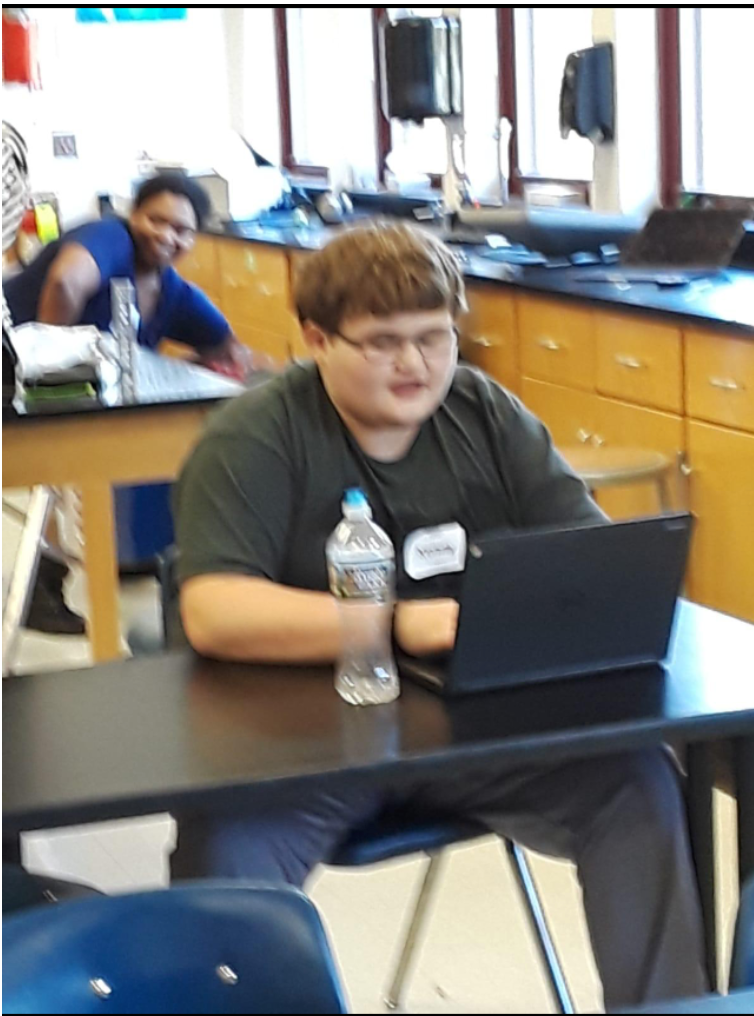
\includegraphics[width=75mm,scale=0.5]{november3/pic1.png}
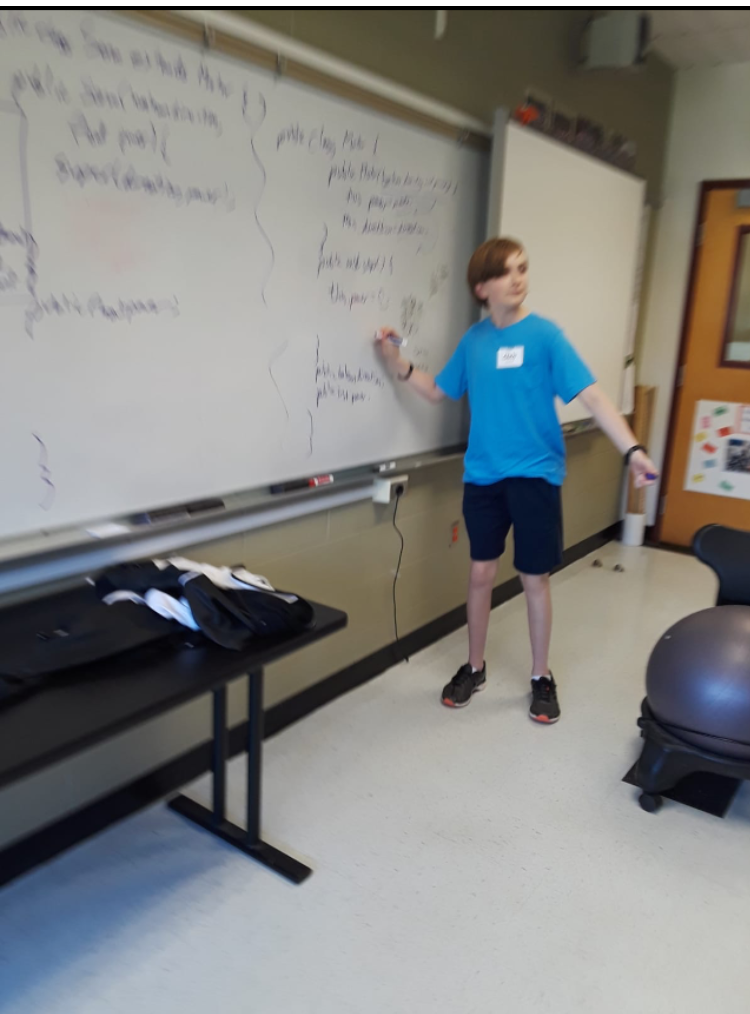
\includegraphics[width=75mm,scale=0.5]{november3/pic2.png}
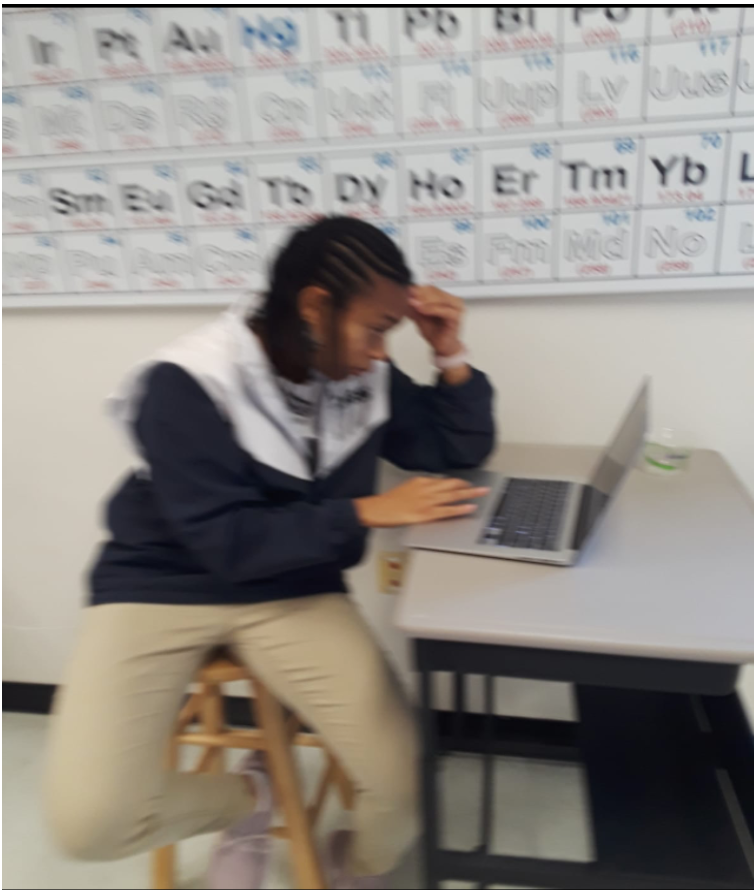
\includegraphics[width=75mm,scale=0.5]{november3/pic3.png}
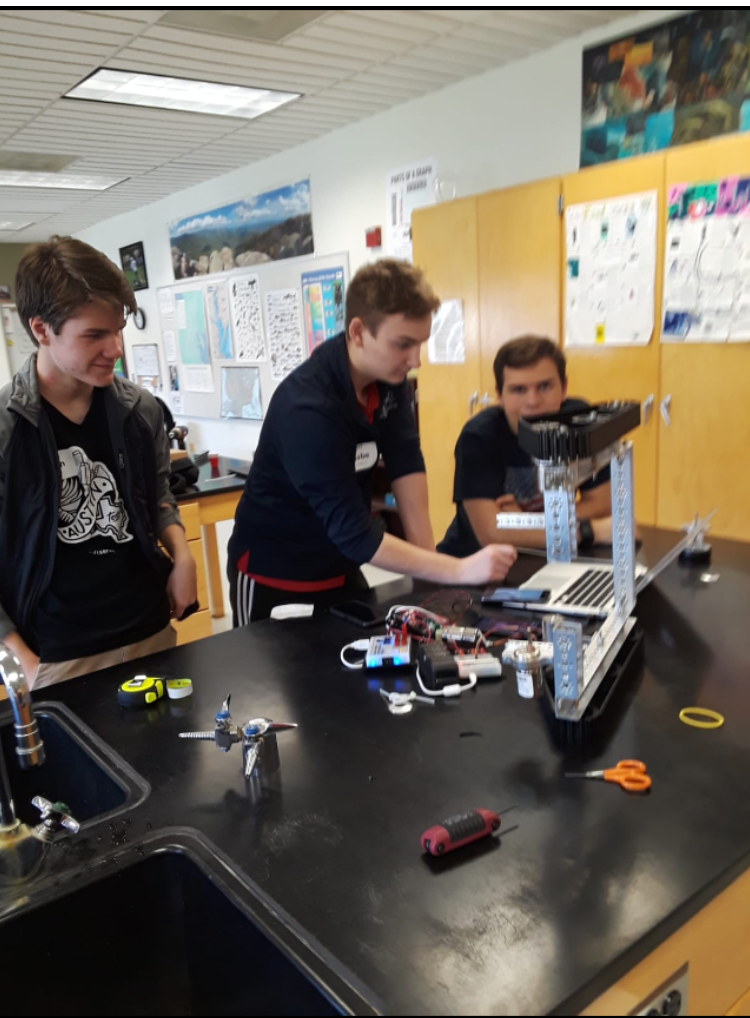
\includegraphics[width=75mm,scale=0.5]{november3/pic4.png}
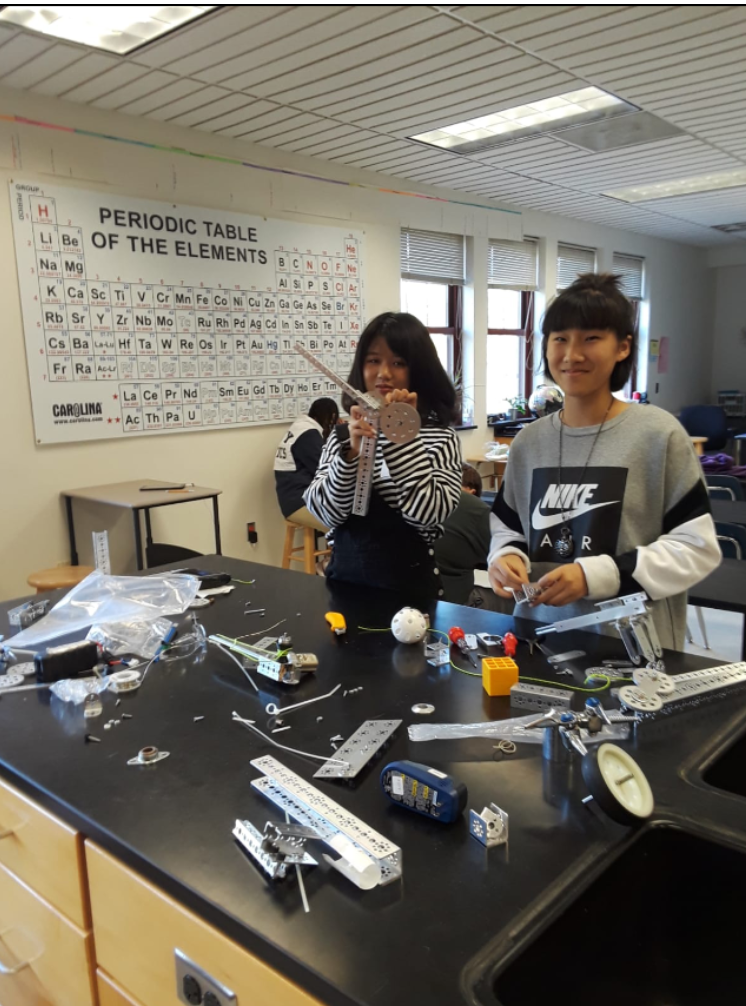
\includegraphics[width=75mm,scale=0.5]{november3/pic5.png}
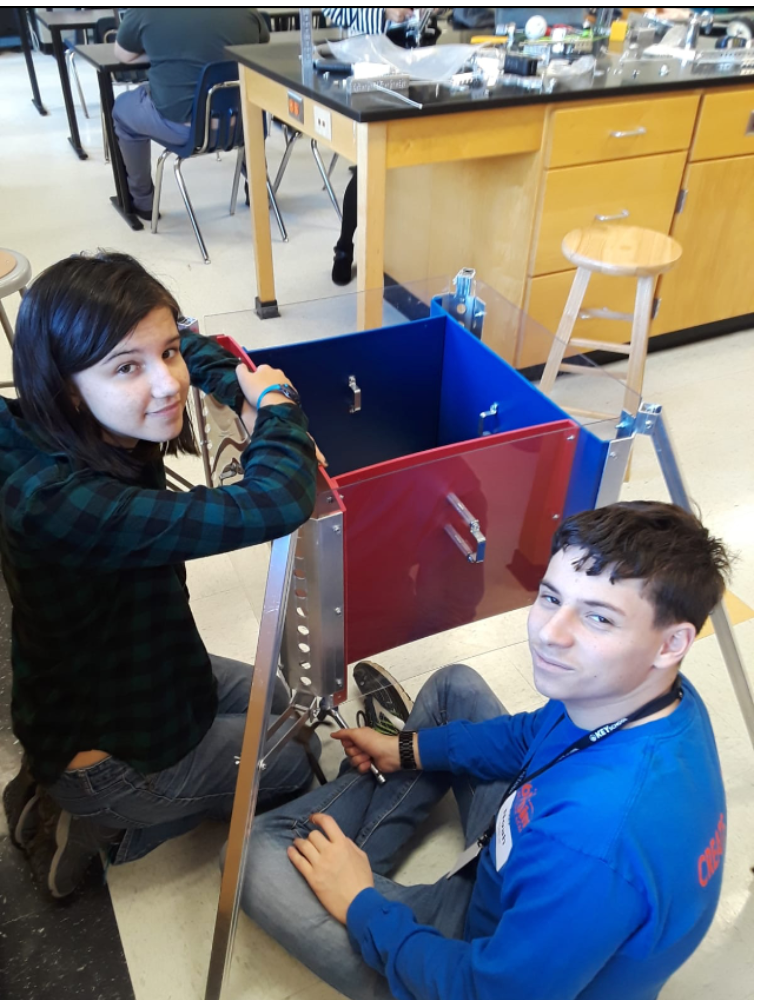
\includegraphics[width=75mm,scale=0.5]{november3/pic6.png}



\end{document}

